% *********************************************************************
% © 2021-2023 Jeremy Sylvestre
%
% Permission is granted to copy, distribute and/or modify this document
% under the terms of the GNU Free Documentation License, Version 1.3 or
% any later version published by the Free Software Foundation; with no
% Invariant Sections, no Front-Cover Texts, and no Back-Cover Texts. A
% copy of the license is included in the appendix entitled “GNU Free
% Documentation License” that appears in the output document of this
% PreTeXt source code. All trademarks™ are the registered® marks of
% their respective owners.
%
% *********************************************************************

\newcommand*{\xmin}{0}
\newcommand*{\xmax}{8}
\newcommand*{\ymin}{-20}
\newcommand*{\ymax}{20}

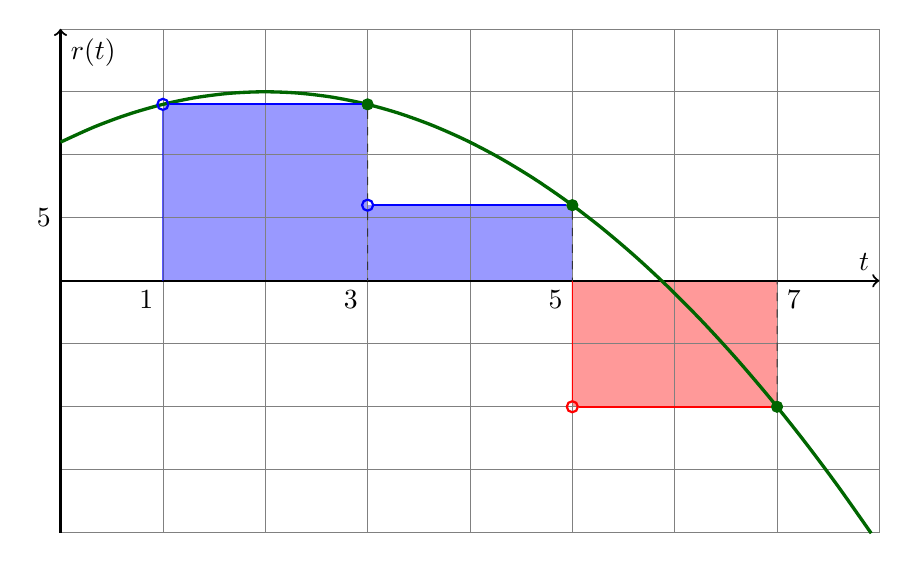
\begin{tikzpicture}
[
	closedpt/.style={circle,draw,fill,inner sep=0pt,minimum size=4pt},
	openpt/.style={circle,draw,inner sep=0pt,minimum size=4pt},
	xscale=1.3,
	yscale=0.16
]

	% rectangle fills
	\fill[blue!40!white] (1,14) rectangle (3,0);
	\fill[blue!40!white] (3,6) rectangle (5,0);
	\fill[red!40!white] (5,-10) rectangle (7,0);

	% grid
	\foreach \x in {0,1,2,...,8} {
		\draw[very thin,gray] (\x,\ymin) -- (\x,\ymax);
	}
	\foreach \y in {-20,-15,-10,...,20} {
		\draw[very thin,gray] (\xmin,\y) -- (\xmax,\y);
	}

	% label grid
	\foreach \x in {1,3,5} {
		\node[below left] at (\x,0) {$\x$};
	}
	\foreach \x in {7} {
		\node[below right] at (\x,0) {$\x$};
	}
	\foreach \y in {5} {
		\node[left] at (0,\y) {$\y$};
	}

	% axes
	\draw[->,thick] (\xmin,0) -- (\xmax,0) node[above left] {$t$};
	\draw[->,thick] (0,\ymin) -- (0,\ymax) node[below right] {$r(t)$};

	% continuous graph
	\draw[green!40!black,very thick,domain=0:7.92,smooth] plot (\x,{- \x * \x + 4 * \x + 11});

	% levels and dividers
	\node[blue,thick,openpt] at (1,14) (start) {};
	\node[green!40!black,closedpt] at (3,14) (stop) {};
	\draw[blue,thick] (start) -- (stop);
	\draw[blue,thin] (start) -- (1,0);
	\node[blue,thick,openpt] at (3,6) (start) {};
	\draw[black!80!white,dashed]
	  (stop) -- (start)
	  (start) -- (3,0)
	;
	\node[green!40!black,closedpt] at (5,6) (stop) {};
	\draw[blue,thick] (start) -- (stop);
	\draw[black!80!white,dashed] (stop) -- (5,0);
	\node[red,thick,openpt] at (5,-10) (start) {};
	\node[green!40!black,closedpt] at (7,-10) (stop) {};
	\draw[red,thick] (start) -- (stop);
	\draw[red,thin] (start) -- (5,0);
	\draw[black!80!white,dashed] (stop) -- (7,0);

\end{tikzpicture}
